% Source PDF page 35 (printed p. 21)
\section{仿射集与凸集}
\subsection{直线与线段}
设 $x_1\ne x_2$ 是 $\R^n$ 中的两点。形如
\[
 y=\theta x_1+(1-\theta)x_2,\qquad \theta\in\R
\]
的点构成经过 $x_1$ 和 $x_2$ 的\emph{直线}。参数值 $\theta=0$ 对应 $y=x_2$，$\theta=1$ 对应 $y=x_1$。$\theta$ 在0与1之间的值对应 $x_1$ 和 $x_2$ 之间的闭\emph{线段}。

将 $y$ 写成
\[
 y=x_2+\theta(x_1-x_2)
\]
可得到另一种解释：$y$ 是基点 $x_2$（对应 $\theta=0$）与方向 $x_1-x_2$ 经参数 $\theta$ 缩放后的和，该方向由 $x_2$ 指向 $x_1$。因此，$\theta$ 表示 $y$ 位于从 $x_2$ 到 $x_1$ 路程的什么比例处。$\theta$ 从0增加到1时，$y$ 从 $x_2$ 移到 $x_1$；$\theta>1$ 时，$y$ 位于直线上越过 $x_1$ 的一侧。图2.1给出了示意。

\subsection{仿射集}
如果集合 $C\subseteq\R^n$ 中任意两个不同点所确定的整条直线都包含在 $C$ 中，就称 $C$ 是\emph{仿射集}。也就是说，对任意 $x_1,x_2\in C$ 和 $\theta\in\R$，都有 $\theta x_1+(1-\theta)x_2\in C$。换言之，只要系数之和为一，$C$ 中任意两点的线性组合仍在 $C$ 中。

这个概念可以推广到两个以上的点。形如 $\theta_1x_1+\cdots+\theta_kx_k$，且 $\theta_1+\cdots+\theta_k=1$ 的点，称为 $x_1,\ldots,x_k$ 的\emph{仿射组合}。由仿射集的定义，即它包含其中任意两点的所有仿射组合，利用归纳法可证明：仿射集包含其中各点的任意仿射组合。也就是说，如果 $C$ 是仿射集，$x_1,\ldots,x_k\in C$，且 $\theta_1+\cdots+\theta_k=1$，那么 $\theta_1x_1+\cdots+\theta_kx_k$ 也属于 $C$。

% Source PDF page 36 (printed p. 22)
\begin{figure}[htbp]\centering
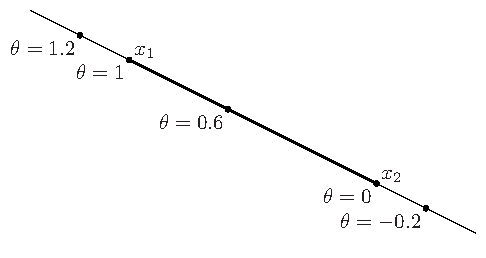
\includegraphics[width=.62\textwidth]{figures/ch02-figure-1.pdf}
\caption*{图2.1\quad 经过 $x_1$ 和 $x_2$ 的直线可参数化为 $\theta x_1+(1-\theta)x_2$，其中 $\theta$ 遍历 $\R$。两点之间的线段对应 $0\le\theta\le1$，图中以深色表示。}
\end{figure}
如果 $C$ 是仿射集，且 $x_0\in C$，那么集合
\[
 V=C-x_0=\{x-x_0\mid x\in C\}
\]
是一个子空间，即对加法与标量乘法封闭。为此，设 $v_1,v_2\in V$，$\alpha,\beta\in\R$。于是 $v_1+x_0\in C$、$v_2+x_0\in C$，从而
\[
 \alpha v_1+\beta v_2+x_0
 =\alpha(v_1+x_0)+\beta(v_2+x_0)+(1-\alpha-\beta)x_0\in C,
\]
因为 $C$ 是仿射集，且 $\alpha+\beta+(1-\alpha-\beta)=1$。由 $\alpha v_1+\beta v_2+x_0\in C$，得到 $\alpha v_1+\beta v_2\in V$。

因此，仿射集 $C$ 可以写成
\[
 C=V+x_0=\{v+x_0\mid v\in V\},
\]
即一个子空间加一个平移量。与仿射集 $C$ 关联的子空间 $V$ 不依赖于 $x_0$ 的选择，因此可以取 $C$ 中任意一点作为 $x_0$。我们将仿射集 $C$ 的\emph{维数}定义为子空间 $V=C-x_0$ 的维数，其中 $x_0$ 为 $C$ 中任意元素。

\begin{origexample}{2.1}
\textbf{线性方程的解集。}线性方程组的解集 $C=\{x\mid Ax=b\}$ 是仿射集，其中 $A\in\R^{m\times n}$、$b\in\R^m$。为证明这一点，设 $x_1,x_2\in C$，即 $Ax_1=b$、$Ax_2=b$。那么对任意 $\theta$，有
\[
\begin{aligned}
 A(\theta x_1+(1-\theta)x_2)
 &=\theta Ax_1+(1-\theta)Ax_2\\
 &=\theta b+(1-\theta)b\\
 &=b.
\end{aligned}
\]
这表明仿射组合 $\theta x_1+(1-\theta)x_2$ 也属于 $C$。与仿射集 $C$ 关联的子空间是 $A$ 的零空间。
\end{origexample}
反过来也成立：每个仿射集都可以表示为某个线性方程组的解集。

% Source PDF page 37 (printed p. 23)
集合 $C\subseteq\R^n$ 中各点的所有仿射组合所成的集合，称为 $C$ 的\emph{仿射包}，记为 $\aff C$：
\[
 \aff C=\{\theta_1x_1+\cdots+\theta_kx_k\mid
 x_1,\ldots,x_k\in C,\ \theta_1+\cdots+\theta_k=1\}.
\]
仿射包是包含 $C$ 的最小仿射集，具体地说：若 $S$ 是满足 $C\subseteq S$ 的任意仿射集，则 $\aff C\subseteq S$。

\subsection{仿射维数与相对内部}
集合 $C$ 的\emph{仿射维数}定义为其仿射包的维数。仿射维数在凸分析和优化中很有用，但不总与其他维数定义一致。例如，考虑 $\R^2$ 中的单位圆周 $\{x\in\R^2\mid x_1^2+x_2^2=1\}$。其仿射包为整个 $\R^2$，故仿射维数为二；但按照大多数维数定义，$\R^2$ 中的单位圆周维数为一。

如果 $C\subseteq\R^n$ 的仿射维数小于 $n$，它便位于仿射集 $\aff C\ne\R^n$ 中。集合 $C$ 的\emph{相对内部}记为 $\relint C$，定义为它相对于 $\aff C$ 的内部：
\[
 \relint C=\{x\in C\mid \text{存在 }r>0, B(x,r)\cap\aff C\subseteq C\},
\]
其中 $B(x,r)=\{y\mid\norm{y-x}\le r\}$ 是关于范数 $\norm{\cdot}$、以 $x$ 为中心、半径为 $r$ 的球。（这里可以使用任意范数，所有范数确定相同的相对内部。）进而可将 $C$ 的\emph{相对边界}定义为 $\cl C\setminus\relint C$，其中 $\cl C$ 是 $C$ 的闭包。

\begin{origexample}{2.2}
考虑 $\R^3$ 的 $(x_1,x_2)$ 平面内的正方形
\[
 C=\{x\in\R^3\mid-1\le x_1\le1,\ -1\le x_2\le1,\ x_3=0\}.
\]
其仿射包为 $(x_1,x_2)$ 平面，即 $\aff C=\{x\in\R^3\mid x_3=0\}$。$C$ 的内部为空，但相对内部为
\[
 \relint C=\{x\in\R^3\mid-1<x_1<1,\ -1<x_2<1,\ x_3=0\}.
\]
它在 $\R^3$ 中的边界是自身；相对边界则是正方形的线框轮廓
\[
 \{x\in\R^3\mid\max\{\abs{x_1},\abs{x_2}\}=1,\ x_3=0\}.
\]
\end{origexample}

\subsection{凸集}
如果 $C$ 中任意两点之间的线段都在 $C$ 中，就称集合 $C$ 是\emph{凸的}。也就是说，对任意 $x_1,x_2\in C$ 以及满足 $0\le\theta\le1$ 的任意 $\theta$，都有
\[
 \theta x_1+(1-\theta)x_2\in C.
\]

% Source PDF page 38 (printed p. 24)
\begin{figure}[htbp]\centering
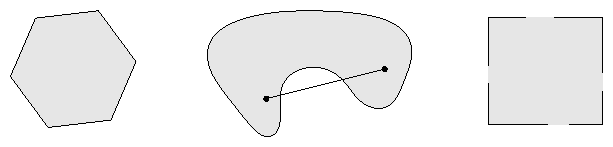
\includegraphics[width=.85\textwidth]{figures/ch02-figure-2.pdf}
\caption*{图2.2\quad 几个简单的凸集与非凸集。左：包含边界（深色线）的六边形是凸集。中：肾形集合不是凸集，因为图中以实点表示的两点之间的线段没有完全包含在集合中。右：正方形包含一部分边界点而不包含另一些边界点，该集合不是凸集。}
\end{figure}
\begin{figure}[htbp]\centering
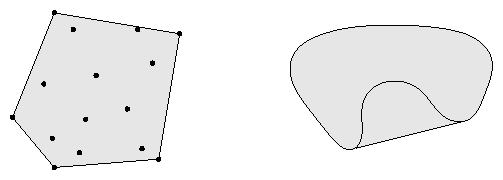
\includegraphics[width=.82\textwidth]{figures/ch02-figure-3.pdf}
\caption*{图2.3\quad $\R^2$ 中两个集合的凸包。左：十五个点（实点）组成的集合，其凸包为阴影所示的五边形。右：图2.2中肾形集合的凸包，为阴影所示的集合。}
\end{figure}
粗略地说，如果集合中任意两点都能沿其间一条没有障碍的直线路径彼此看见，这个集合就是凸的；这里“没有障碍”是指路径始终在集合中。每个仿射集都是凸集，因为它包含任意两个不同点之间的整条直线，当然也包含两点之间的线段。图2.2给出 $\R^2$ 中几个简单的凸集和非凸集。

形如 $\theta_1x_1+\cdots+\theta_kx_k$，且满足 $\theta_1+\cdots+\theta_k=1$、$\theta_i\ge0$（$i=1,\ldots,k$）的点，称为 $x_1,\ldots,x_k$ 的\emph{凸组合}。与仿射集类似，可以证明：一个集合是凸集，当且仅当它包含其中各点的任意凸组合。点的凸组合可理解为这些点的混合或加权平均，$\theta_i$ 表示 $x_i$ 在混合中所占的比例。

集合 $C$ 的\emph{凸包}记作 $\conv C$，是 $C$ 中各点的所有凸组合构成的集合：
\[
 \conv C=\{\theta_1x_1+\cdots+\theta_kx_k\mid
 x_i\in C,\ \theta_i\ge0,\ i=1,\ldots,k,\ \theta_1+\cdots+\theta_k=1\}.
\]
顾名思义，凸包 $\conv C$ 总是凸集。它是包含 $C$ 的最小凸集：若 $B$ 是任意包含 $C$ 的凸集，则 $\conv C\subseteq B$。图2.3说明了凸包的定义。

凸组合的概念可推广至无穷级数、积分，以及最一般的概率分布形式。

% Source PDF page 39 (printed p. 25)
设 $\theta_1,\theta_2,\ldots$ 满足
\[
 \theta_i\ge0,\quad i=1,2,\ldots,\qquad \sum_{i=1}^{\infty}\theta_i=1,
\]
且 $x_1,x_2,\ldots\in C$，其中 $C\subseteq\R^n$ 凸。如果级数收敛，则
\[
 \sum_{i=1}^{\infty}\theta_i x_i\in C.
\]
更一般地，设 $p:\R^n\to\R$ 对所有 $x\in C$ 满足 $p(x)\ge0$，且 $\int_Cp(x)\,\mathrm dx=1$，其中 $C\subseteq\R^n$ 凸。如果积分存在，则
\[
 \int_C p(x)x\,\mathrm dx\in C.
\]
最一般的形式如下：设 $C\subseteq\R^n$ 凸，随机向量 $x$ 以概率一属于 $C$，则 $\E x\in C$。事实上，其他形式都包含在这一形式中。例如，设随机变量 $x$ 只取 $x_1$ 和 $x_2$ 两个值，且 $\Prob(x=x_1)=\theta$、$\Prob(x=x_2)=1-\theta$，其中 $0\le\theta\le1$。那么 $\E x=\theta x_1+(1-\theta)x_2$，又回到了简单的两点凸组合。

\subsection{锥}
若对每个 $x\in C$ 和 $\theta\ge0$ 都有 $\theta x\in C$，就称集合 $C$ 为\emph{锥}，或称其\emph{非负齐次}。若 $C$ 既是凸集又是锥，就称其为\emph{凸锥}；也就是说，对任意 $x_1,x_2\in C$ 和 $\theta_1,\theta_2\ge0$，有
\[
 \theta_1x_1+\theta_2x_2\in C.
\]
从几何上看，这种形式的点构成一个二维扇形，顶点在原点，两条边分别经过 $x_1$ 和 $x_2$，见图2.4。

形如 $\theta_1x_1+\cdots+\theta_kx_k$，且 $\theta_1,\ldots,\theta_k\ge0$ 的点，称为 $x_1,\ldots,x_k$ 的\emph{锥组合}或\emph{非负线性组合}。若 $x_i$ 属于凸锥 $C$，则它们的任意锥组合都在 $C$ 中。反过来，集合 $C$ 是凸锥，当且仅当它包含其元素的所有锥组合。与凸组合、仿射组合一样，锥组合也可推广至无穷级数与积分。

集合 $C$ 的\emph{锥包}是 $C$ 中各点的所有锥组合构成的集合，即
\[
 \{\theta_1x_1+\cdots+\theta_kx_k\mid x_i\in C,\ \theta_i\ge0,\ i=1,\ldots,k\}.
\]
它也是包含 $C$ 的最小凸锥，见图2.5。

% Source PDF page 40 (printed p. 26)
\begin{figure}[htbp]\centering
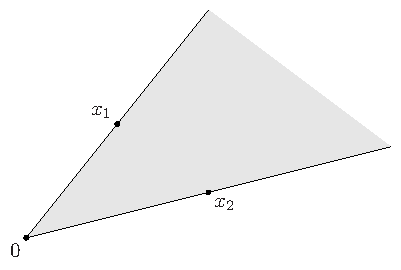
\includegraphics[width=.62\textwidth]{figures/ch02-figure-4.pdf}
\caption*{图2.4\quad 扇形表示所有形如 $\theta_1x_1+\theta_2x_2$、$\theta_1,\theta_2\ge0$ 的点。顶点在原点，对应 $\theta_1=\theta_2=0$；两条边分别对应 $\theta_1=0$ 或 $\theta_2=0$，经过 $x_1$ 和 $x_2$。}
\end{figure}
\begin{figure}[htbp]\centering
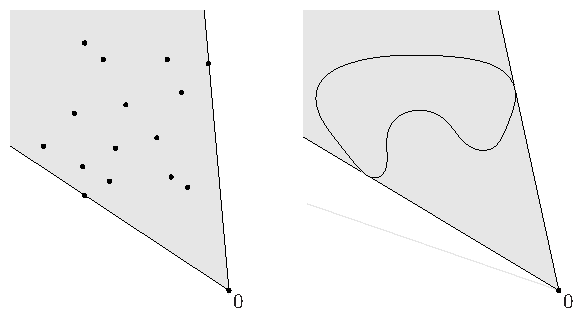
\includegraphics[width=.82\textwidth]{figures/ch02-figure-5.pdf}
\caption*{图2.5\quad 图2.3中两个集合的锥包，以阴影表示。}
\end{figure}

% Source PDF page 41 (printed p. 27)
\section{一些重要例子}
本节介绍一些重要的凸集例子，它们将在本书后续部分反复出现。先从几个简单例子开始。
\begin{itemize}
\item 空集 $\varnothing$、任意单点集 $\{x_0\}$ 以及整个空间 $\R^n$，都是 $\R^n$ 的仿射子集，因此也是凸子集。
\item 任意直线都是仿射集。如果经过原点，它还是子空间，因此也是凸锥。
\item 线段是凸集，但不是仿射集，除非退化为一个点。
\item 形如 $\{x_0+\theta v\mid\theta\ge0\}$、$v\ne0$ 的射线是凸集，但不是仿射集。如果基点 $x_0=0$，它是凸锥。
\item 任意子空间都是仿射集，也是凸锥，因此是凸集。
\end{itemize}

\subsection{超平面与半空间}
\emph{超平面}是形如
\[
 \{x\mid a^{\T}x=b\}
\]
的集合，其中 $a\in\R^n$、$a\ne0$、$b\in\R$。从解析角度看，它是关于 $x$ 各分量的一个非平凡线性方程的解集，因而是仿射集。从几何角度看，超平面 $\{x\mid a^{\T}x=b\}$ 可解释为与给定向量 $a$ 的内积为常数的点集，也可看作法向量为 $a$ 的超平面；常数 $b\in\R$ 确定超平面相对原点的偏移。将超平面写成
\[
 \{x\mid a^{\T}(x-x_0)=0\},
\]
便可理解这一几何解释，其中 $x_0$ 是超平面上任意一点，即满足 $a^{\T}x_0=b$ 的任意点。这个表示还可写成
\[
 \{x\mid a^{\T}(x-x_0)=0\}=x_0+a^{\perp},
\]
其中 $a^{\perp}$ 表示 $a$ 的正交补，即与它正交的所有向量构成的集合：
\[
 a^{\perp}=\{v\mid a^{\T}v=0\}.
\]
这表明，超平面由偏移量 $x_0$ 加上所有与法向量 $a$ 正交的向量构成。图2.6说明了这些几何解释。

一个超平面将 $\R^n$ 分成两个\emph{半空间}。闭半空间是形如
\begin{equation}
 \{x\mid a^{\T}x\le b\}\tag{2.1}
\end{equation}
的集合，其中 $a\ne0$，也就是一个非平凡线性不等式的解集。半空间是凸集，但不是仿射集，见图2.7。

% Source PDF page 42 (printed p. 28)
\begin{figure}[htbp]\centering
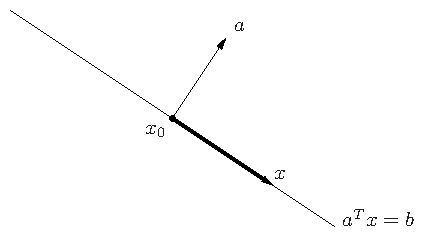
\includegraphics[width=.58\textwidth]{figures/ch02-figure-6.pdf}
\caption*{图2.6\quad $\R^2$ 中的超平面，法向量为 $a$，$x_0$ 为超平面上一点。对超平面上任意点 $x$，向量 $x-x_0$（深色箭头）都与 $a$ 正交。}
\end{figure}
\begin{figure}[htbp]\centering
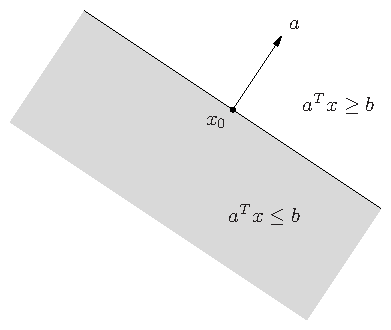
\includegraphics[width=.58\textwidth]{figures/ch02-figure-7.pdf}
\caption*{图2.7\quad $\R^2$ 中由 $a^{\T}x=b$ 定义的超平面确定两个半空间。$a^{\T}x\ge b$ 确定的半空间（无阴影）沿 $a$ 方向延伸；$a^{\T}x\le b$ 确定的半空间（阴影）沿 $-a$ 方向延伸，向量 $a$ 是这个半空间的外法向量。}
\end{figure}

% Source PDF page 43 (printed p. 29)
\begin{figure}[htbp]\centering
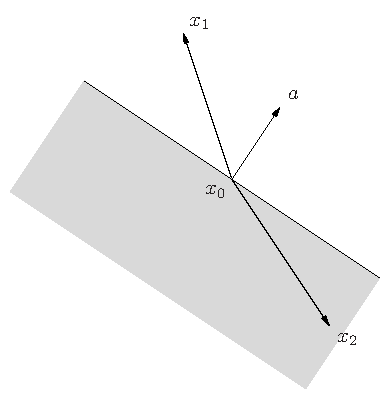
\includegraphics[width=.62\textwidth]{figures/ch02-figure-8.pdf}
\caption*{图2.8\quad 阴影集合是 $a^{\T}(x-x_0)\le0$ 确定的半空间。向量 $x_1-x_0$ 与 $a$ 的夹角为锐角，所以 $x_1$ 不在半空间中；向量 $x_2-x_0$ 与 $a$ 的夹角为钝角，所以 $x_2$ 在半空间中。}
\end{figure}
半空间（2.1）还可表示为
\begin{equation}
 \{x\mid a^{\T}(x-x_0)\le0\},\tag{2.2}
\end{equation}
其中 $x_0$ 是相应超平面上的任意一点，即满足 $a^{\T}x_0=b$。表示（2.2）给出一个简单的几何解释：半空间由 $x_0$ 加上所有与外法向量 $a$ 成钝角或直角的向量构成，如图2.8所示。

半空间（2.1）的边界是超平面 $\{x\mid a^{\T}x=b\}$。集合 $\{x\mid a^{\T}x<b\}$ 是半空间 $\{x\mid a^{\T}x\le b\}$ 的内部，称为\emph{开半空间}。

\subsection{欧几里得球与椭球}
$\R^n$ 中的\emph{欧几里得球}，简称\emph{球}，具有形式
\[
 B(x_c,r)=\{x\mid\norm{x-x_c}_2\le r\}
 =\{x\mid(x-x_c)^{\T}(x-x_c)\le r^2\},
\]
其中 $r>0$，$\norm{\cdot}_2$ 表示欧几里得范数，即 $\norm u_2=(u^{\T}u)^{1/2}$。向量 $x_c$ 是球心，标量 $r$ 是半径；$B(x_c,r)$ 包含距球心 $x_c$ 不超过 $r$ 的所有点。欧几里得球的另一种常见表示为
\[
 B(x_c,r)=\{x_c+ru\mid\norm u_2\le1\}.
\]

% Source PDF page 44 (printed p. 30)
\begin{figure}[htbp]\centering
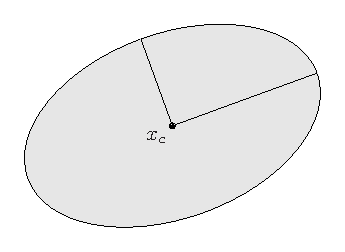
\includegraphics[width=.58\textwidth]{figures/ch02-figure-9.pdf}
\caption*{图2.9\quad $\R^2$ 中的椭球，以阴影表示。中心 $x_c$ 以实点表示，两条半轴以线段表示。}
\end{figure}
欧几里得球是凸集：若 $\norm{x_1-x_c}_2\le r$、$\norm{x_2-x_c}_2\le r$，且 $0\le\theta\le1$，则
\[
\begin{aligned}
 \norm{\theta x_1+(1-\theta)x_2-x_c}_2
 &=\norm{\theta(x_1-x_c)+(1-\theta)(x_2-x_c)}_2\\
 &\le\theta\norm{x_1-x_c}_2+(1-\theta)\norm{x_2-x_c}_2\\
 &\le r.
\end{aligned}
\]
这里使用了 $\norm{\cdot}_2$ 的齐次性和三角不等式，见第A.1.2节。与球相关的另一族凸集是\emph{椭球}，其形式为
\begin{equation}
 \mathcal E=\{x\mid(x-x_c)^{\T}P^{-1}(x-x_c)\le1\},\tag{2.3}
\end{equation}
其中 $P=P^{\T}\succ0$，即 $P$ 对称正定。向量 $x_c\in\R^n$ 是椭球中心，矩阵 $P$ 确定椭球从 $x_c$ 沿各方向延伸的程度；椭球 $\mathcal E$ 的半轴长度为 $\sqrt{\lambda_i}$，其中 $\lambda_i$ 是 $P$ 的特征值。球是 $P=r^2I$ 的椭球。图2.9给出 $\R^2$ 中的一个椭球。

椭球的另一种常见表示是
\begin{equation}
 \mathcal E=\{x_c+Au\mid\norm u_2\le1\},\tag{2.4}
\end{equation}
其中 $A$ 是非奇异方阵。在这个表示中，不失一般性，可以假设 $A$ 对称正定。取 $A=P^{1/2}$，便得到（2.3）定义的椭球。如果（2.4）中的 $A$ 对称半正定但奇异，则（2.4）所示集合称为\emph{退化椭球}；其仿射维数等于 $A$ 的秩。退化椭球也为凸集。

\subsection{范数球与范数锥}
设 $\norm{\cdot}$ 是 $\R^n$ 上的任意范数，见第A.1.2节。由范数的一般性质可证明，以 $x_c$ 为中心、$r$ 为半径的范数球 $\{x\mid\norm{x-x_c}\le r\}$ 是凸集。与范数 $\norm{\cdot}$ 关联的\emph{范数锥}为
\[
 C=\{(x,t)\mid\norm x\le t\}\subseteq\R^{n+1}.
\]
